% Template for ICASSP-2018 paper; to be used with:
%          spconf.sty  - ICASSP/ICIP LaTeX style file, and
%          IEEEbib.bst - IEEE bibliography style file.
% --------------------------------------------------------------------------
\documentclass{article}
\usepackage{spconf,amsmath,graphicx}

% Example definitions.
% --------------------
\def\x{{\mathbf x}}
\def\L{{\cal L}}

% Title.
% ------
\title{Gaussian Mixture Model for Voice Conversion}
%
% Single address.
% ---------------

\name{Caleb Kaiji Lu  \and \textit{Tyler Nuanes} \and \textit{Nanshu Wang} \and \textit{Serhan Oztekin}}
\address{Carnegie Mellon University\\School of Electrical and Computer Engineering\\23, NASA Research Park, Moffett Field, CA 94035}
%
% For example:
% ------------
%\address{School\\
%	Department\\
%	Address}
%
% Two addresses (uncomment and modify for two-address case).
% ----------------------------------------------------------
%\twoauthors
%  {A. Author-one, B. Author-two\sthanks{Thanks to XYZ agency for funding.}}
%	{School A-B\\
%	Department A-B\\
%	Address A-B}
%  {C. Author-three, D. Author-four\sthanks{The fourth author performed the work
%	while at ...}}
%	{School C-D\\
%	Department C-D\\
%	Address C-D}
%
\begin{document}
%\ninept
%
\maketitle

\begin{abstract}
Voice conversion is defined as modifying a source speaker’s voice to sound as though it were produced by a target speaker, a problem challenging enough  that a fully successful algorithm has so far proved elusive. Speech signals are created in a complex process involving vibrations of vocal chords and frequency filtering by the vocal tract. In addition, our auditory process is nonlinear, involving multiple frequency bands in the cochlea. Humans pick up characteristics of individual voices in frequencies ranging from 3 Hz to 10 kHz. Instead of attempting to develop a new algorithm, we focused our project on delving into a fundamental algorithm in the field and worked to reproduce it. Our training set includes 150 parallel audios from a female source and a male target. The results show that the \textit{MelCD}, a measure of distortion, of Full Conversion is 37.66,  and \textit{MelCD} of VQ Conversion is 39.53. The Full Conversion reduced  \textit{MelCD} by 4.77 dB compared to the original distortion between source and target, a significant improvement. 
\end{abstract}
%
\begin{keywords}
voice conversion, signal processing, machine learning
\end{keywords}
\section{Introduction}
\label{sec:intro}
Voice conversion technology can have applications ranging from entertainment to speaker recognition. It would be beneficial to the media industry to reproduce the voices of famous actors or actresses after they have passed. It would also be useful in translating media to different languages in the original actress or actor's voice. It may also help in the grieving process—--how many people wish they could hear a loved one’s voice one last time after they pass? Voice conversion research can also contribute to fundamental research in other areas--for instance, achieving voice conversion means voice identification must be possible.

A fair amount of work has been done on this topic. For example, some methods propose to learn source--target relationship from a number utterances \cite{stylianou2009voice}, some methods are parametric, which learns a mapping function between a source to target in some feature spaces\cite{stylianou1998continuous}\cite{kawahara1997speech}.An alternative approach is called unit selection\cite{duxans2006voice}\cite{jin2016cute}. The idea is to select the segments from training sets of a target voice, which correspond to the speech content of source voice, then concatenating the seg- ments with smooth transition.

Our contribution is an implementation of the voice conversion work-flow algorithm given by Stylianou et al \cite{stylianou1998continuous}. In short this involves feature extraction of the fundamental frequency $f_0$ and mel's cepstrum $mcep$, dynamic time wrapping (DTW) to align the speech of our target and source speaker in the training data, conversion to the target voice using VQ and Full Conversion algorithms with Gaussian Mixture Models, $F_0$ transformation to match the fundamental frequency to the target speaker, and reproduction of an audio signal. We wrap up our report by evaluating of distortion as a measure of performance. 


\section{Background}
\label{sec:background}
This section will focus on describing the fundamental principles behind our voice conversion algorithm. It will describe human voice differentiation, the human auditory response in conjunction with the mel frequency bank and Mel cepstrums, the Dynamic Time Warping algorithm, and a description of Gaussian Mixture Models.
\subsection{Human Voice Production and Identification}

Unfortunately for voice conversion technology, speakers have a variety of individual characteristics that affect their speech. Human vocal tract and speaking patterns are highly individualized and humans have evolved a strong ability to discriminate between different speakers \cite{latinus2011human}.  Speaking rate, pitch contour, etc are all important features that help to identify individual speakers. However, some of the most significant characteristics of speaker identity are embedded in the statistical distribution of the speech envelope\cite{reynolds1995robust}. Based on this concept and previous work, we will focus on voice conversion using the speech envelope as our primary feature.

Of additional importance is the distinction between ``voiced'' and ``unvoiced'' frequencies. Voiced sounds are produced by vocal cords, have more amplitude, and can be represented by near-constant frequencies of a particular duration. The maximum voiced frequency tends to be cut off at about 4 kHz. Above this range, there are ``unvoiced'' sounds, which are non-periodic sounds caused by air pressed through a constricted vocal tract. Due to the aperiodic and short-time nature of such events, they tend to have more frequency components which also tend to be higher\cite{bachu2008separation}. Studies have shown voiced speech to play a larger role in speaker individuality than unvoiced speech \cite{stylianou1998continuous}, so our conversion will focus on the voiced portions of speech.

\subsection{Human Auditory Response and the Mel Frequency Bank}
Human auditory response further complicates analysis and reconstruction of speech. Specifically, human perception of pitch, or frequency, follows a nonlinear scale. When humans judge whether pitches are equal distances from one another, they select frequencies over larger and larger intervals, starting around 500 Hz. In addition, the same sound amplitude over a range of frequencies will have different perceived loudness levels over those frequencies. Based on these phenomenon, the Mel scale was developed\cite{ghosh2012comparative}. A Mel-filter bank can be created to simulate the filtering occurring in the human auditory system with a series of overlapping triangular bandpass filters, centered on the Mel frequencies. 
\begin{figure}[htb]

\begin{minipage}[b]{1.0\linewidth}
  \centering
  \centerline{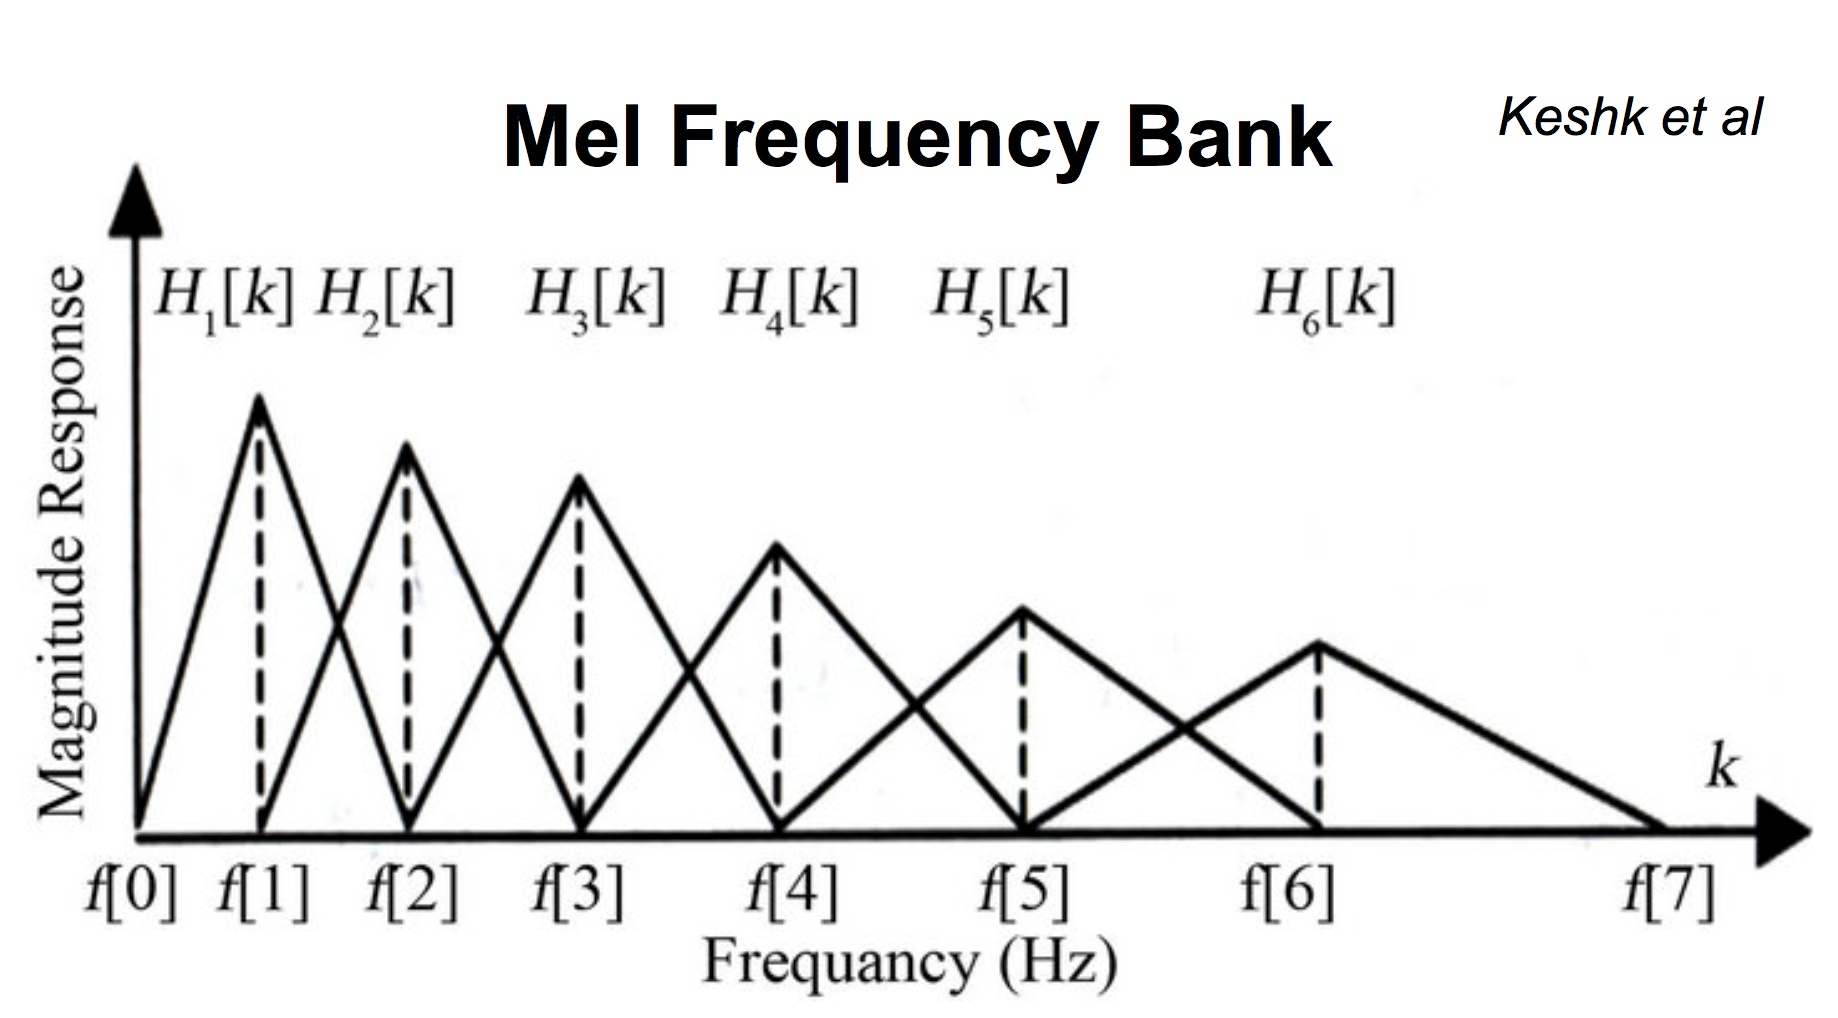
\includegraphics[width=8.5cm]{image6}}
%  \vspace{2.0cm}
\end{minipage}
% %
% \begin{minipage}[b]{.48\linewidth}
%   \centering
%   \centerline{\includegraphics[width=4.0cm]{image3}}
% %  \vspace{1.5cm}
%   \centerline{(b) Results 3}\medskip
% \end{minipage}
% \hfill
% \begin{minipage}[b]{0.48\linewidth}
%   \centering
%   \centerline{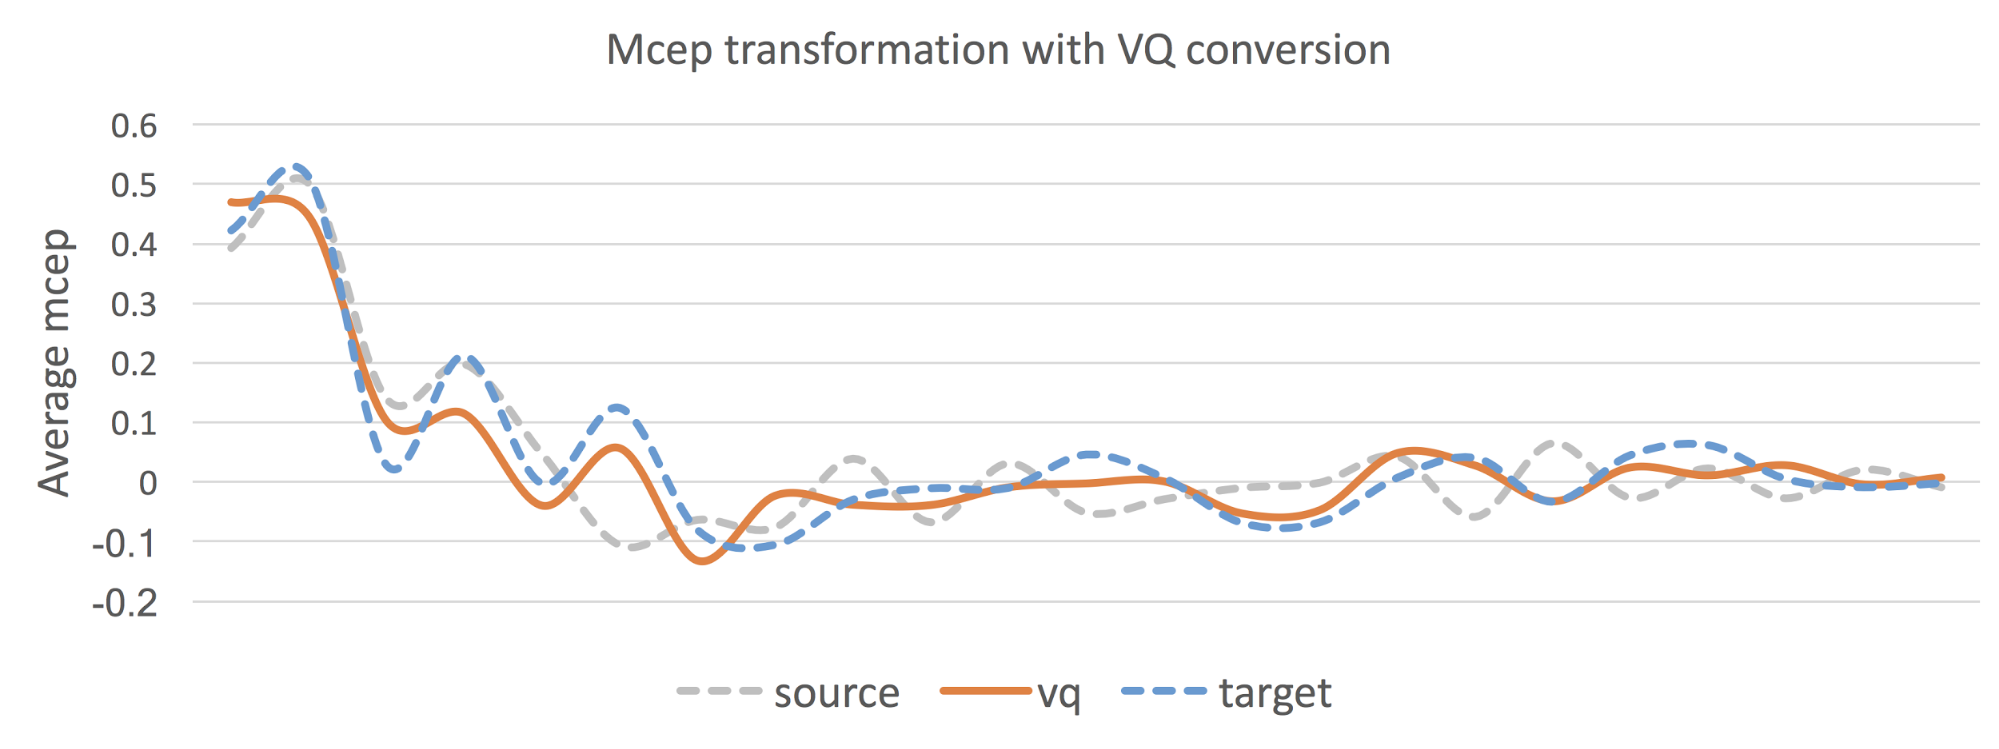
\includegraphics[width=4.0cm]{image4}}
% %  \vspace{1.5cm}
%   \centerline{(c) Result 4}\medskip
% \end{minipage}
% %
\caption{Mel frequency bank}
\label{fig:melfrequency}
%
\end{figure}

When using the Mel Frequency bank to imitate the human auditory response, first the Fourier Transform of the speech signal is taken to transform the signal to the time domain. Next, the Mel Frequency Bank is applied as a filter to the frequency-domain signal. Then the logarithm is taken across all frequencies to convert the spectrum into a dB scale. The frequencies are filtered out above 4 kHz, to keep only the voiced frequencies in the signal. Finally, the Discrete Cosine Transform is taken, converting the signal to Mel-Frequency Cepstral Coefficients (MFCC's), which will be referred to as Mel's cepstrum throughout this paper.

\subsection{Dynamic Time Warping}

Before feeding the features for training, target and source speaker's cepstrums should be aligned using Dynamic Time Warping(DTW), a nonlinear method of finding optimal alignment between two time-series data \cite{ratanamahatana2004everything}. The algorithm computes the matrix of distances between each two points, as shown below.
\begin{align*}
C_t = |mc^t_{source} - mc^t_{target}|
\end{align*}

\begin{figure}[htb]

\begin{minipage}[b]{1.0\linewidth}
  \centering
  \centerline{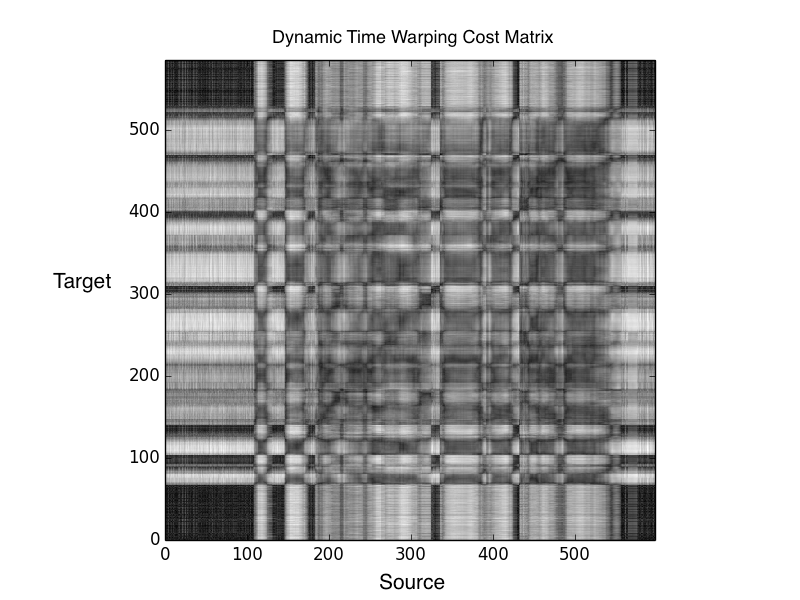
\includegraphics[width=8.5cm]{image9}}
%  \vspace{2.0cm}
\end{minipage}
\caption{The distance matrix between source and target data}
\label{fig:costmatrix}
%
\end{figure}

To discover the warp, it find the path through the matrix that minimizes the total cumulative distances between the two sequences. The algorithm is fairly straightforward. First, the (0,0) point’s value is kept the same. Then, it assigns each cell along the first column the running sum of the elements below it:
\begin{align*}
    D(0,m) = \sum_{k=0}^m c(0,y_k)
\end{align*}
Similarly, it assigns each cell along the first row the running sum of the elements before it.
\begin{align*}
    D(n,0) = \sum_{k=0}^n c(x_k,0)
\end{align*}
Finally, it iteratively selects the smallest value from the cells to the left, below, and diagonal left-below, summing that value with the value in the current cell.
\begin{align*}
    D(n,m) &= min\{D(n-1,m-1),D(n-1,m),D(n,m-1)\} \\
    &+c(x_n,y_m)
\end{align*}
This creates the accumulated cost matrix and allows for efficient calculation of the best path.

\begin{figure}[htb]

\begin{minipage}[b]{1.0\linewidth}
  \centering
  \centerline{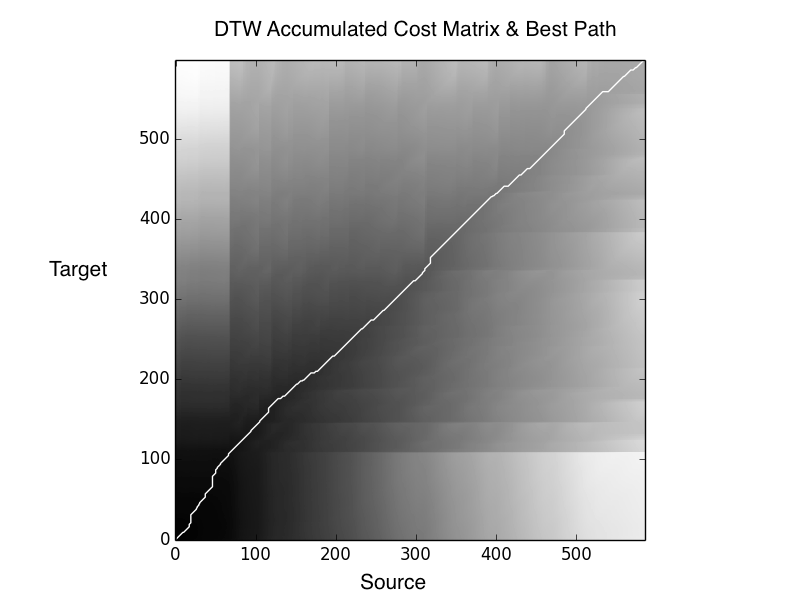
\includegraphics[width=8.5cm]{image10}}
%  \vspace{2.0cm}
\end{minipage}
\caption{The accumulated cost matrix and the best path}
\label{fig:accucostmatrix}
%
\end{figure}

\subsection{Gaussian Mixture Model}
A Gaussian Mixture Model represents the data as a weighted sum of Gaussian distributions, each with a characteristic mean and variance. Gaussian Mixture Models (GMMs) have been shown to be a reliable choice for voice conversion because Mel's cepstrums can be represented as a mixture of multiple Gaussian components\cite{stylianou1998continuous}. We will elaborate on their use in the next section.
\section{Approach}
\label{sec:pagestyle}
\begin{figure*}[t]
  \centering
  \centerline{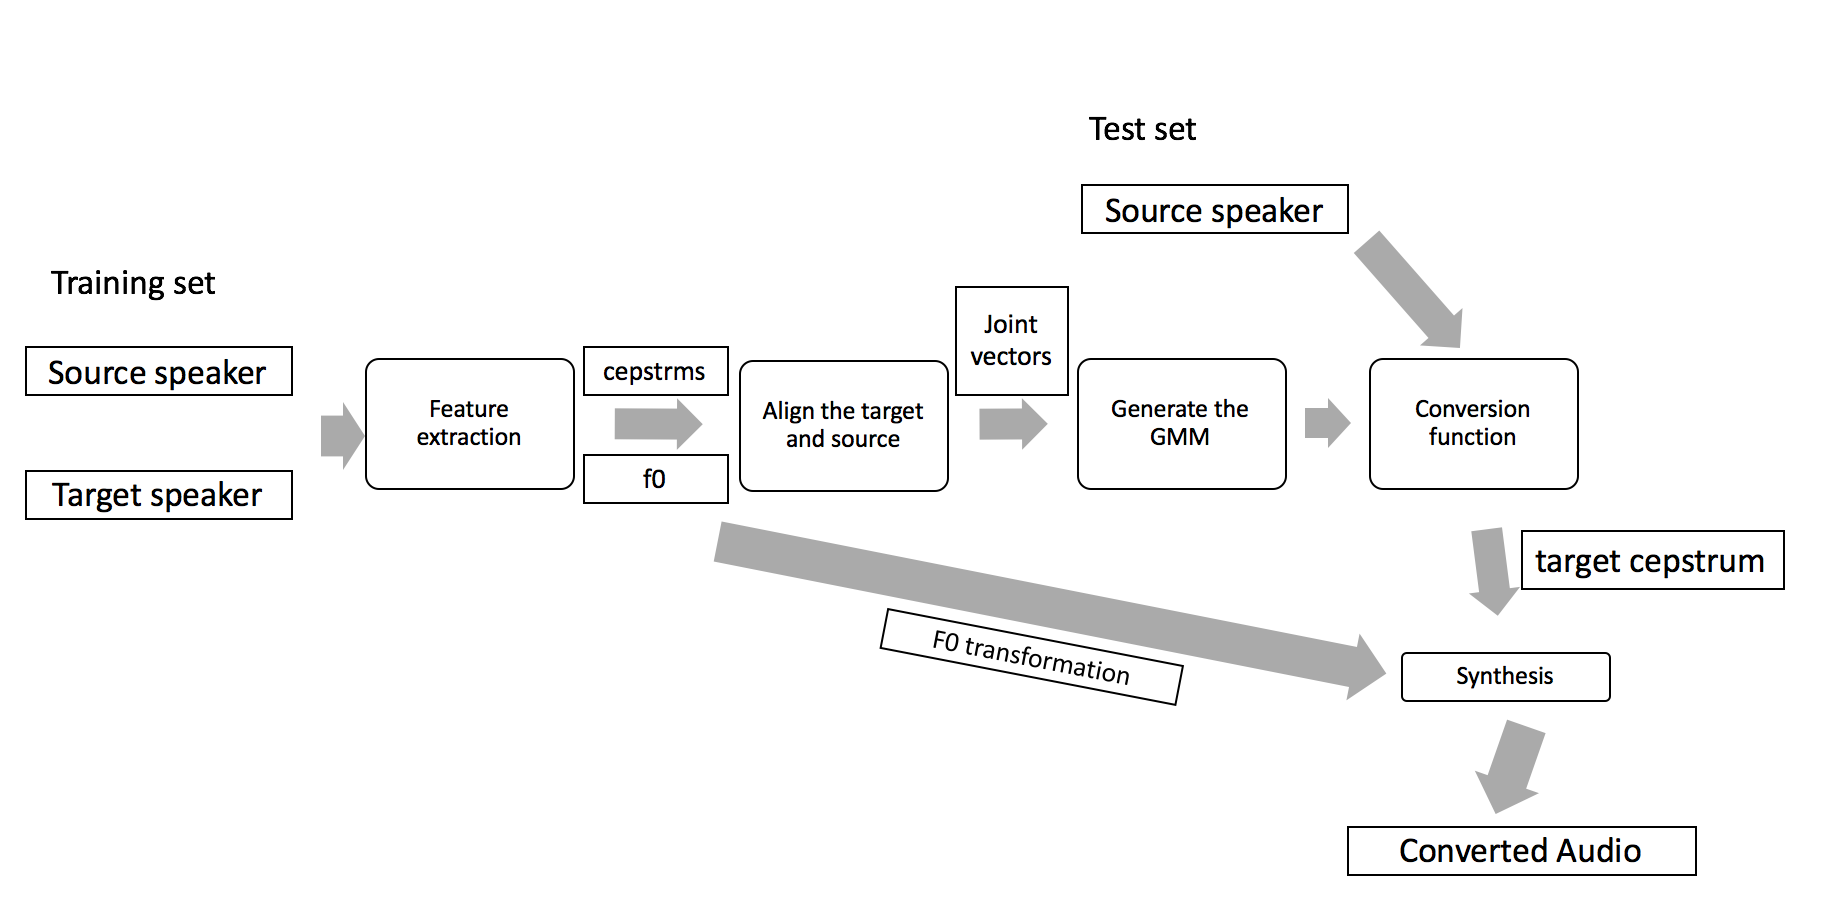
\includegraphics[width=\linewidth]{image11}}
%  \vspace{2.0cm}
\caption{The algorithm flowchart}
\label{fig:algorithm}
%
\end{figure*}

Based on the complexity of this field and the duration of our project, we chose to implement an algorithm based on a foundational paper in the field. Specifically, Stylianou's foundational work\cite{stylianou1998continuous}, on which more advanced voice conversion technology is based. In this section, we will cover in detail our approach of the feature extraction for cepstrums and fundamental frequency, the alignment of the source and target feature using dynamic time warping, and the use of GMM in training with 2 different conversion functions. 

\subsection{Dataset and Software}We used the dataset from VCC2016\cite{toda2016voice}, which contains 5 source speakers and 5 target speakers. Each speaker utters the same sentence set of 162 sentences. We selected 160 sentences from one source speaker and one sentence speaker. Of the 160 pairs of sentences,  150 pairs of them are used for training and 10 for testing. The sampling rate is 16 kHz, and stored in 16-bit format. Various python libraries were used for the purpose of this project including \texttt{dtw}, \texttt{pyworld}, \texttt{pysptk}, and \texttt{sklearn}.

\subsection{Feature Extraction}
Using a time step of $5ms$, we extracted 25 mel-frequency cepstrums from each time step.
\subsection{Alignment}
We implemented the Dynamic Time Warping(DTW) method mentioned in the background section to generate the aligned features for the source and target features.
\subsection{GMM}
The basic idea is to train GMMs for the joint vector features for source and target spectral features. EM algorithm with Maximum Likelihood Estimation iteratively generates a GMM for the aligned features of the source and target. 
Once we have the GMMs models, the next step is to use GMMs for converting source features to target features. The GMM conversion function deserves special treatment due to its complexity. The primary component of the conversion function is a conditional probability built on the GMM. From the GMM, it is possible to calculate the probability of a target cepstrum given the source speech cepstrum. 
\begin{align*}
    p(x) = \sum_{i=1}^m \alpha_i N(x;\mu_i,\Sigma_i)
\end{align*}

The paper by Stylianou\cite{stylianou1998continuous} proposes and compares three different conversion methods: Full, Diagonal, and VQ Conversion. In our work, we implemented Full and VQ conversion for comparison. Each class in the GMM model is defined by its parameters: mean and variance. As a result, different posteriori conversion functions can be used to convert target to source based on the GMM components and their parameters. VQ only considers only the mean target vector, whereas Full also considers the cross-covariance matrix of source and target vectors, which acts as a correction term to achieve the minimum mean-squared error.
\begin{align*}
    \text{VQ Conversion:}\\
    F(x_t) &= \sum_{i=1}^m P(C_i|x_t)\nu_i \\
    \text{Full Conversion:}\\
    F(x_t) &= \sum_{i=1}^m P(C_i|x_t)[\nu_i + \Gamma_i\Sigma_i^{-1}(x_t-\mu_i)] \\
\end{align*}
Where $\nu$  is the mean target vector and $\Gamma$ is the cross-covariance matrix between source and target.
Since Full conversion is more complicated but is the more accurate model, the following table shows the comparison of the two conversion functions:
\begin{center}
    \begin{tabular}{ | c | c | c |}
    \hline
    Conversion & Performance & Computation \\\hline
    VQ & poor & simple\\ \hline
    Full & best & costly\\ \hline
    % Diagonal & better than VQ & better than Full\\ \hline
    \end{tabular}
\end{center}   
\subsection{Algorithm}
In conclusion, the algorithm can be described as follows and in Figure \ref{fig:algorithm}:
\begin{enumerate}
\item Calculate the Mel cepstrum
\item Align the target and source speaker's cepstrums
\item Generate the GMM on source and target training data
\item Convert a source cepstrum to the matching target cepstrum using the conversion function
\item Convert the cepstrum back to speech audio:
\begin{enumerate}
\item Convert the cepstrum to the frequency domain.
\item Match the average fundamental frequency to the target.
\item Convert the spectrogram back to the time domain.
\end{enumerate}
\end{enumerate}

\section{Results}
\label{sec:results}

After converting speech from the source speaker to target speaker, we evaluated our resort as a measure of relative distortion, according to the equation below \cite{mashimo2001evaluation}.

\begin{align*}
    MelCD = \frac{10}{\ln10}\sqrt{2\sum^{25}_{i=1}(mc_i^{conv} - mc_i^{tar})^2}
\end{align*}

Essentially, this equation gives the dB scale of distortion between two Mel Cepstrums. First, we calculate the original distortion between the target and source for the same phrase. Then we calculate the difference between the converted voice and the target for VQ and Full Conversion, as shown in Figure \ref{fig:melcd} below. The results show that the \textit{MelCD}, a measure of distortion, of Full Conversion is 37.66,  and \textit{MelCD} of VQ Conversion is 39.53. The Full Conversion reduced  \textit{MelCD} by 4.77 dB compared to the original distortion between source and target, which is significant. The following two images are Figure \ref{fig:vqresult} and Figure \ref{fig:fullresult}, which display the envelope of the source, target, and converted speech for VQ and Full Conversion, respectively.

\begin{figure}[htb]
  \centering
  \centerline{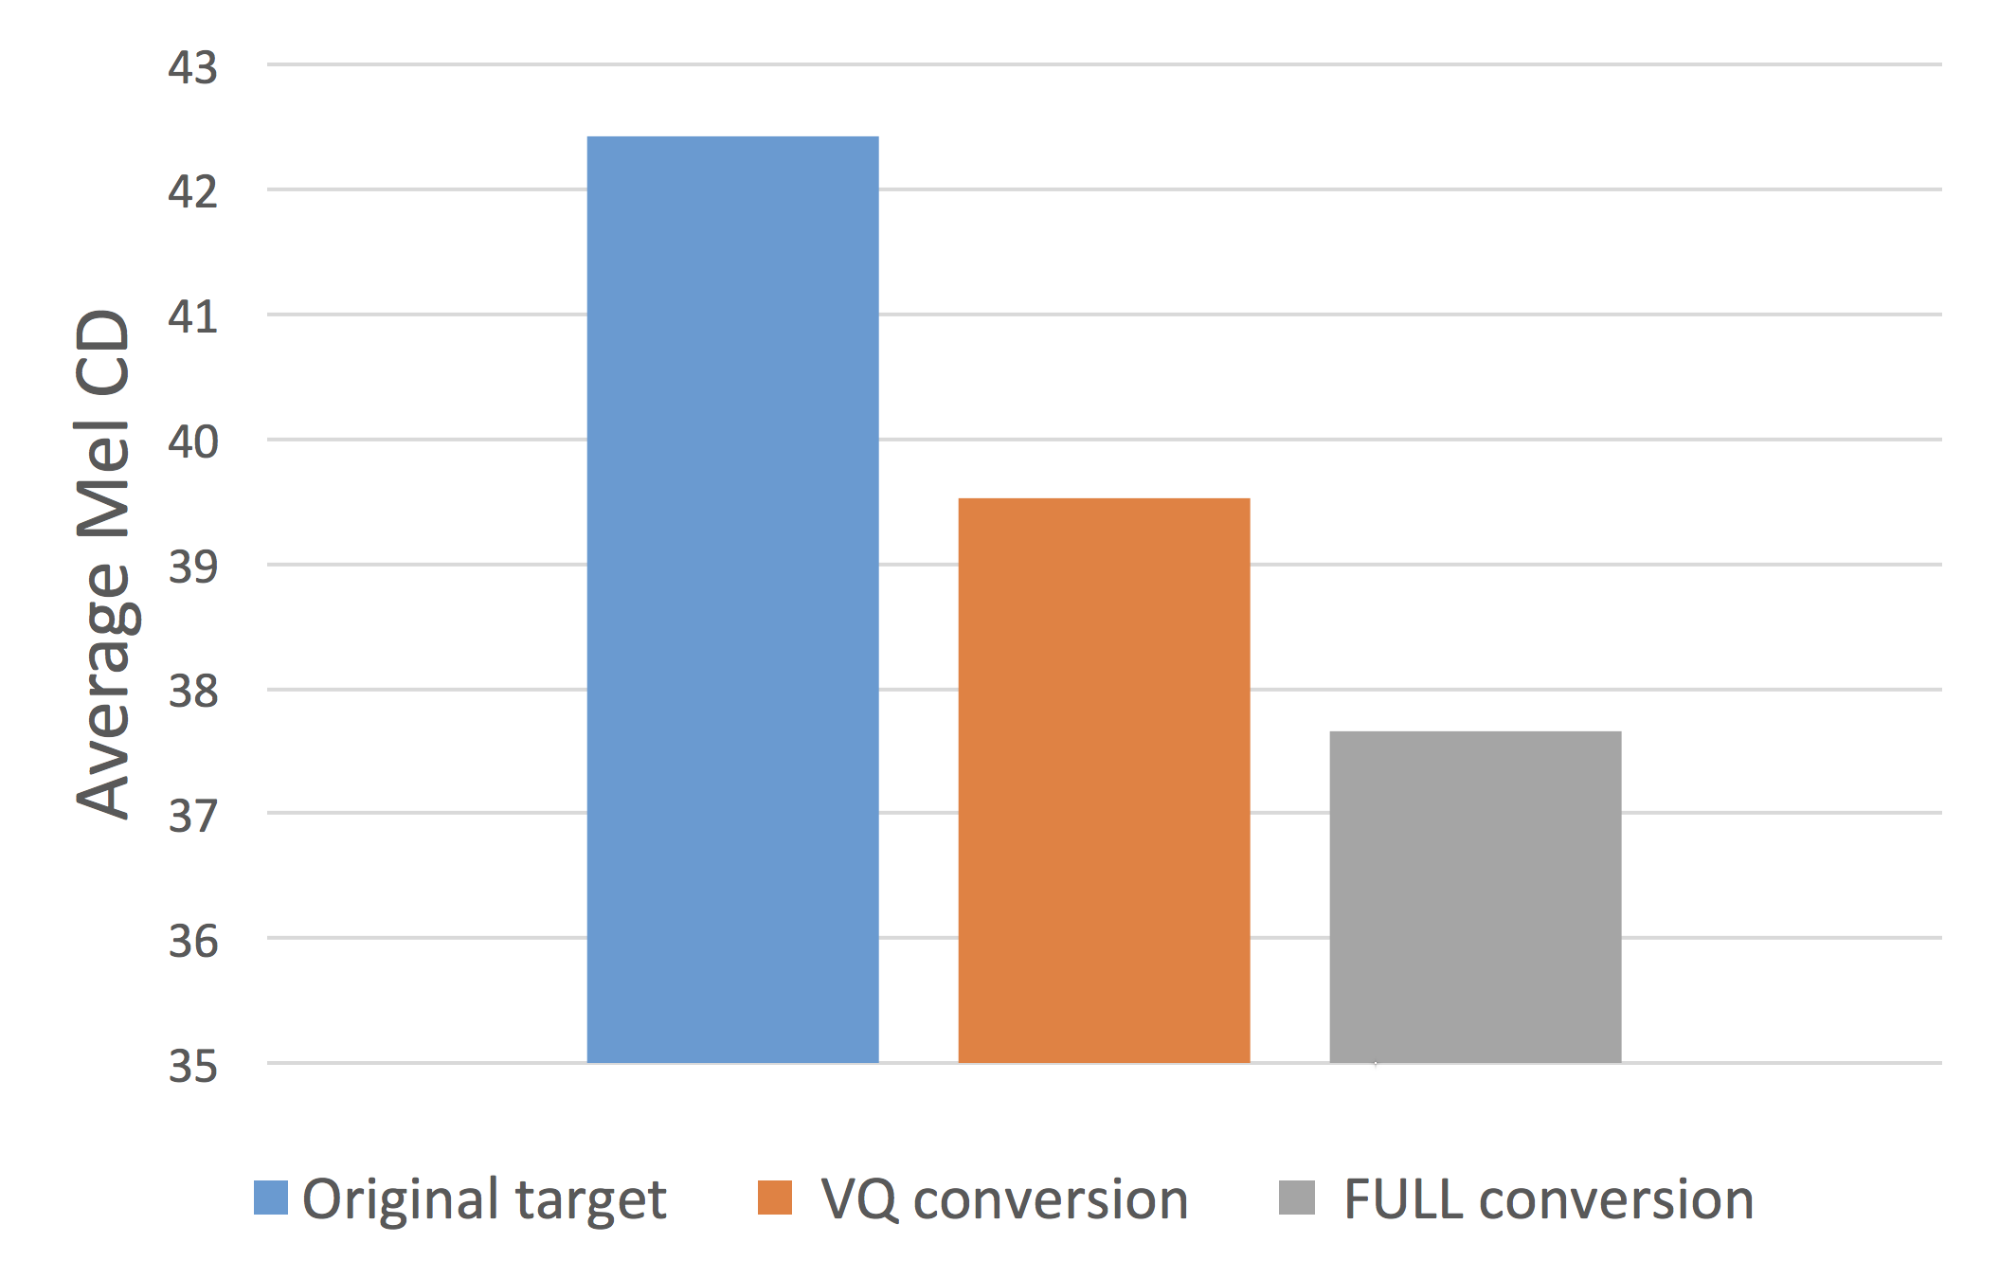
\includegraphics[width=8.5cm]{image2}}
%  \vspace{2.0cm}
\caption{The MelCD comparison of no conversion, full conversion and VQ conversion}
\label{fig:melcd}
%
\end{figure}

\begin{figure}[htb]
\begin{minipage}[b]{1\linewidth}
  \centering
  \centerline{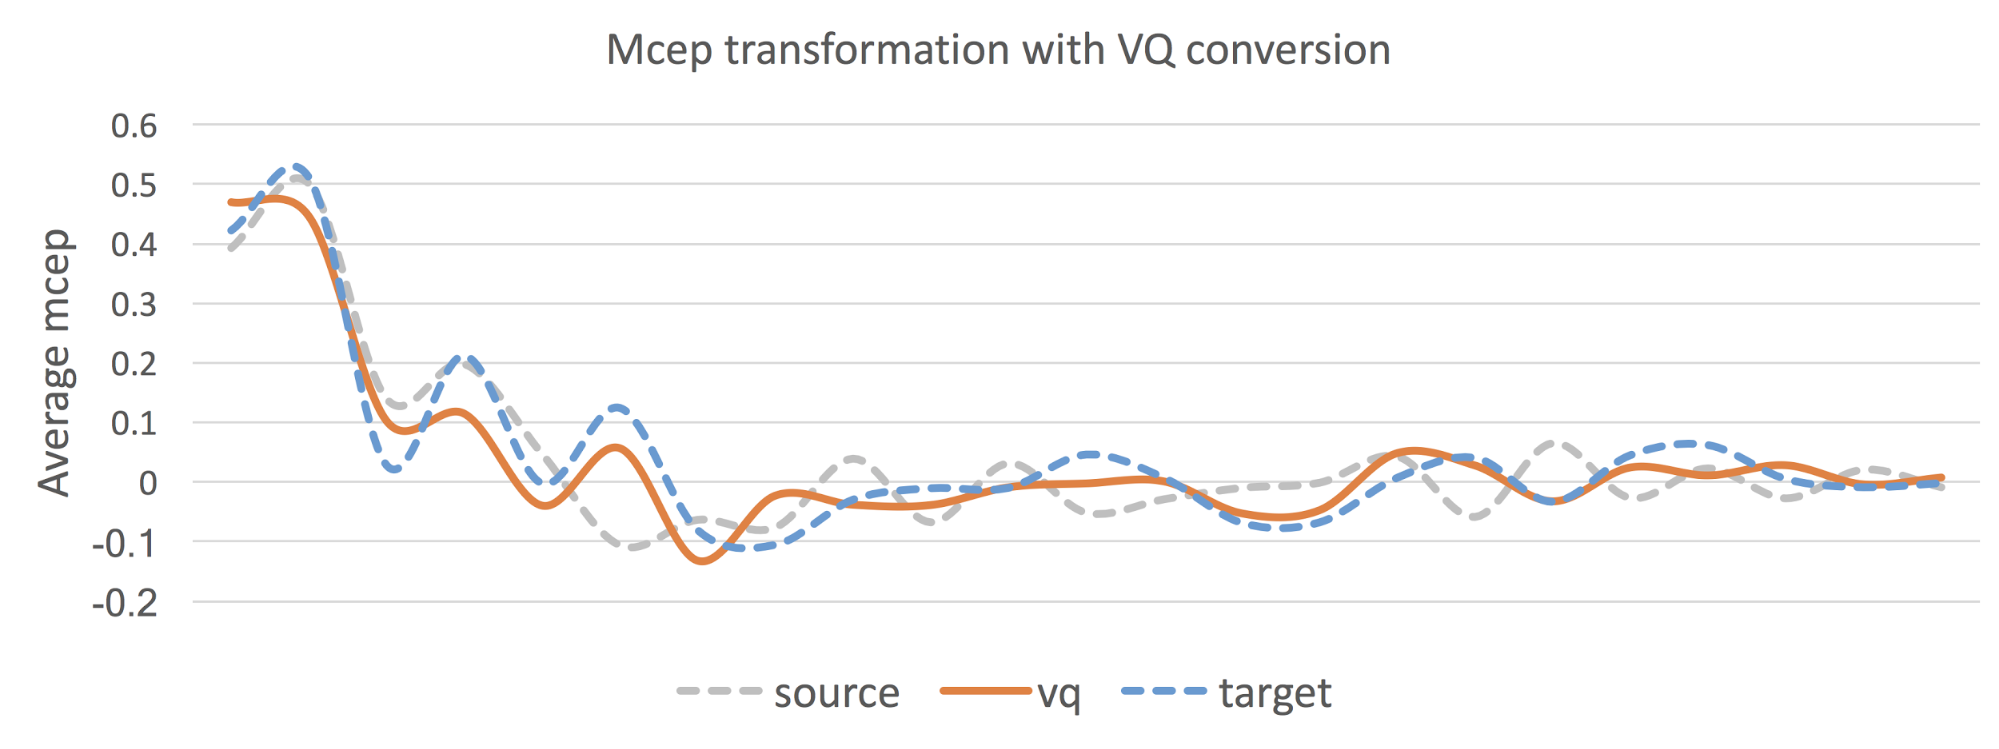
\includegraphics[width=8.5cm]{image4}}
%  \vspace{2.0cm}
\end{minipage}
\caption{Average mcep values for VQ conversion.}
\label{fig:vqresult}
\end{figure}

\begin{figure}[htb]
\begin{minipage}[b]{1\linewidth}
  \centering
  \centerline{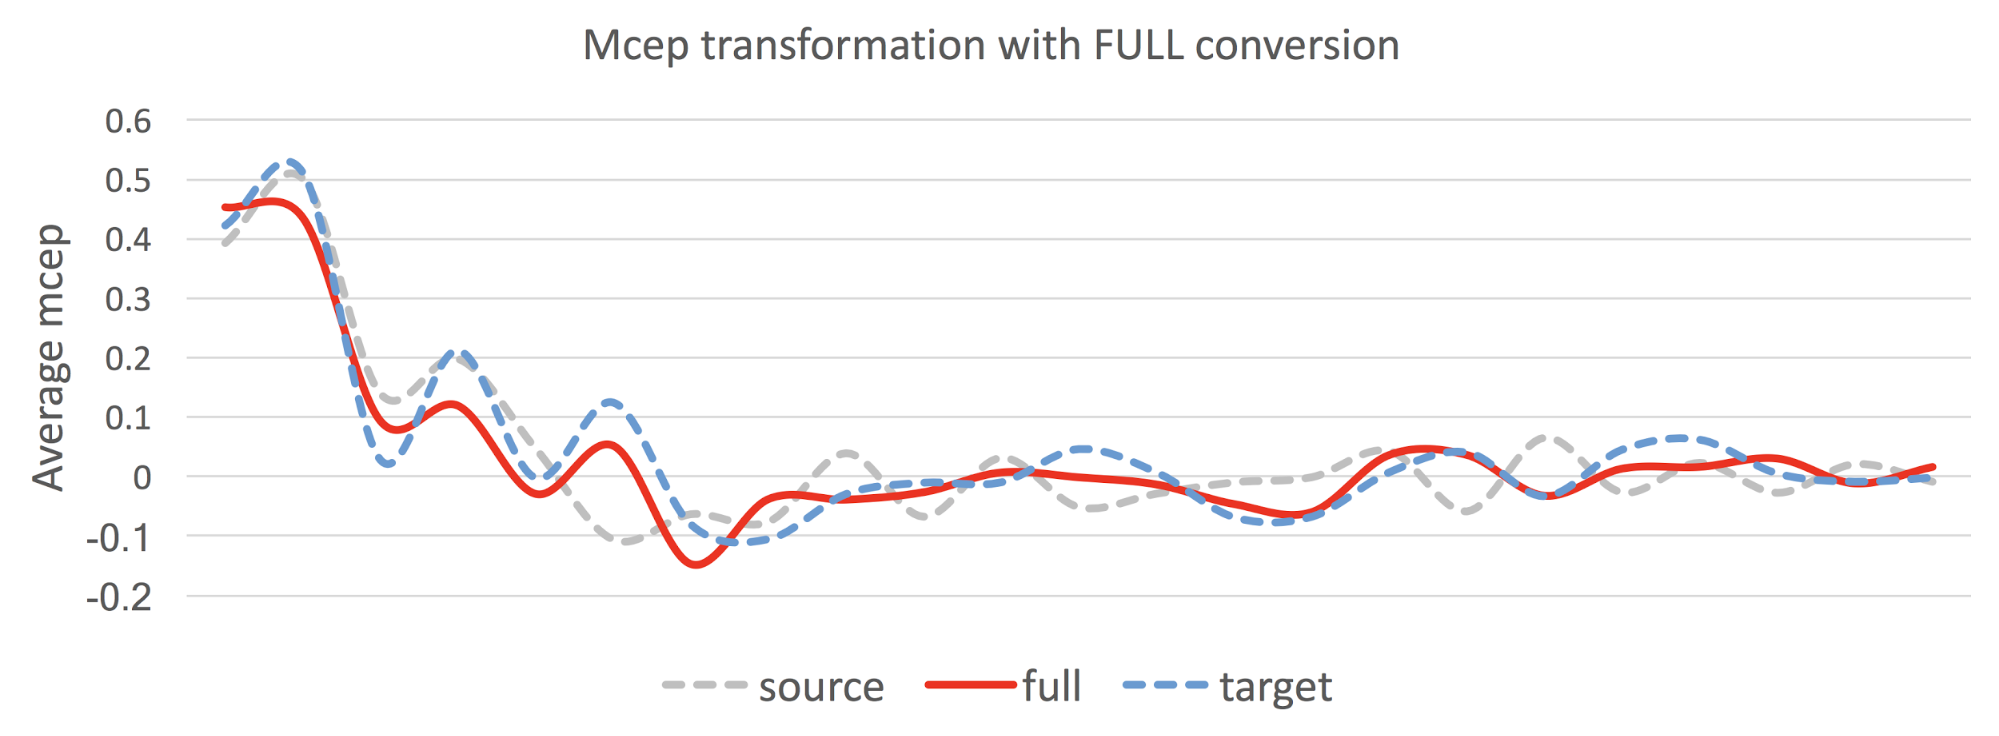
\includegraphics[width=8.5cm]{image5}}
%  \vspace{1.5cm}
\end{minipage}

\caption{Average mcep values for Full conversion.}
\label{fig:fullresult}
%
\end{figure}
\section{Conclusion}
\label{sec:conclusion}


Our work is an implementation of the voice conversion work-flow described by Stylianou et al \cite{stylianou1998continuous}. We extracted the fundamental frequency $f_0$, calculated Mel-frequency cepstrum $mcep$, performed dynamic time wrapping (DTW) to align the speech of our target and source speaker in the training data, calculated VQ and Full Conversion algorithms using Gaussian Mixture Models, and finally performed the $F_0$ transformation to match the fundamental frequency to the target speaker. Our training set includes 150 parallel audios from a female source and a male target, while we have a separate test set for evaluation. Our test data has some fairly impressive results. Future work would first build upon our current results by implementing improvements found in several papers that base their work on Stylianou et al. We may then begin work to improve their algorithms, perhaps by focusing more on unvoiced frequencies or lower-frequency components, such as the rhythm of the speech.

The source code of our project is hosted on GitHub at \url{https://github.com/caleblu/MLSP-Project-fall17}.




% References should be produced using the bibtex program from suitable
% BiBTeX files (here: strings, refs, manuals). The IEEEbib.bst bibliography
% style file from IEEE produces unsorted bibliography list.
% -------------------------------------------------------------------------

\bibliographystyle{IEEEbib}

 
\bibliography{references}

\end{document}
